%----------------------------------------------------------------
%
%  File    :  survey.tex
%
%  Author  :  Keith Andrews, ISDS, TU Graz, Austria
%
%  Created :  24 Mar 2010
%
%  Changed :  22 Nov 2016
%
%----------------------------------------------------------------


\documentclass[11pt,onecolumn,twoside]{report}

\usepackage[          % set page and margin sizes
  a4paper,
  twoside,
  top=5mm,
  bottom=10mm,
  inner=15mm,
  outer=15mm,
  bindingoffset=10mm,
  head=10mm,
  foot=10mm,
  headsep=15mm,
  footskip=15mm,
  includeheadfoot,
]{geometry}
% A4 is 210 x 297 mm



\usepackage{txfonts}            % new times fonts
\usepackage{relsize}            % relative font sizes \smaller \larger

\usepackage[T1]{fontenc}        % 8-bit output chars (must be before inputenx)
\usepackage[utf8]{inputenx}     % input char encoding

\usepackage{float}              % H for float placement
\usepackage{setspace}           % line spacing

\usepackage{textcomp}           % symbols such as \texttimes and \texteuro
\usepackage{latexsym}

\usepackage{siunitx}            % prettier number formatting
\sisetup{%
  group-separator={,},
}
\usepackage[super]{nth}         % 1st, 2nd, 3rd, etc.

\usepackage{xspace}
\usepackage{etoolbox}           % for \newrobustcmd
\usepackage{makecmds}           % for \makecommand
\usepackage{placeins}		   % for FloatBarrier command


\usepackage[english,austrian,british]{babel}

\usepackage{tabu}

\usepackage[bf,sf]{titlesec}



\setlength{\textfloatsep}{10mm plus 2mm minus 1mm}
\setlength{\floatsep}{10mm plus 2mm minus 1mm}
\setlength{\intextsep}{10mm plus 2mm minus 1mm}

\setlength{\dbltextfloatsep}{10mm plus 2mm minus 1mm}
\setlength{\dblfloatsep}{10mm plus 2mm minus 1mm}

\setlength{\abovecaptionskip}{4mm plus 2mm minus 1mm}
\setlength{\belowcaptionskip}{0mm}



% sensible settings for floats
% See http://www-rohan.sdsu.edu/~aty/bibliog/latex/floats.html
% See https://robjhyndman.com/hyndsight/latex-floats/

\setcounter{topnumber}{2}               % max num floats at top of page
\setcounter{dbltopnumber}{2}            % max num floats on 2col page
\setcounter{bottomnumber}{2}            % max num floats at bottom of page
\setcounter{totalnumber}{4}             % max num floats on a page

\renewcommand{\topfraction}{0.8}        % max fraction of floats at top
\renewcommand{\dbltopfraction}{0.9}     % max fraction of floats at top 2col
\renewcommand{\bottomfraction}{0.8}     % max fraction of floats at bottom
\renewcommand{\textfraction}{0.2}       % min fraction of text

% only for entirely float pages:
\renewcommand{\floatpagefraction}{0.7}      % min page fraction having floats
\renewcommand{\dblfloatpagefraction}{0.7}   % min 2col page fraction having floats






% use caption and subfig (caption2 and subfigure are now obsolete)

\usepackage[
  position=bottom,
  margin=1cm,
  font=small,
  labelfont={bf,sf},
  format=hang,
  indention=0mm,
]{caption,subfig}

\captionsetup[subfigure]{
  margin=0pt,
  parskip=0pt,
  hangindent=0pt,
  indention=0pt,
  singlelinecheck=true,
}




% fancyhdr to make nice headers and footers
% and deal with long chapter names

\usepackage{fancyhdr}         % headers and footers
\pagestyle{fancy}             % must call to set defaults before redefining

\renewcommand{\chaptermark}[1]{%
  \markboth{\thechapter.\ #1}{}
}
\renewcommand{\sectionmark}[1]{%
  \markright{\thesection.\ #1}
}
\renewcommand{\headrulewidth}{0mm}
\renewcommand{\footrulewidth}{0mm}
\newcommand{\headlook}{\sffamily}
\fancyhf{}
\fancyhead[LE,RO]{\thepage}
\fancyhead[LO]{%
\parbox[t]{0.8\textwidth}{\headlook\nouppercase{\rightmark}}
}
\fancyhead[RE]{%
\parbox[t]{0.8\textwidth}{\raggedleft\headlook\nouppercase{\leftmark}}
}


%\fancypagestyle{plain}{%   redefine plain style, but doesn't work
%  \fancyhf{}    % clear all header and footer fields
%  \fancyfoot[C]{\headlook \thepage} % except the center
%  \renewcommand{\headrulewidth}{0pt}
%  \renewcommand{\footrulewidth}{0pt}
%}



\usepackage{xcolor}
\definecolor{darkgreen}{rgb}{0.0,0.2,0.0}
\definecolor{darkblue}{rgb}{0.0,0.0,0.2}
\definecolor{darkred}{rgb}{0.2,0.0,0.0}
\definecolor{verylightgrey}{gray}{0.95}
\definecolor{lightgrey}{gray}{0.9}
\definecolor{black}{gray}{0.0}


\usepackage{tabularx}


\usepackage{listings}                 % for listings of source code
\usepackage{calc}                     % for calculation below

\makeatletter
\newlength{\numwidth}%
\setlength{\numwidth}{\widthof{\normalfont{\lst@numberstyle{99}}}}% Up to 2-digit (99) line numbers
\def\lst@PlaceNumber{%
  \makebox[\numwidth+1em][l]{%
    \makebox[\numwidth][r]{\normalfont\lst@numberstyle{\thelstnumber}}%
  }%
}
\makeatother

\lstset{                              % set parameters for listings
  floatplacement=tp,                  % default float placement
  numberbychapter,
  inputencoding=utf8,
  language=,                          % empty = plain text
  basicstyle=\small\ttfamily,
  tabsize=2,
  xleftmargin=1cm,
  xrightmargin=1cm,
  frame=none,
  framexleftmargin=0mm,
  rulesepcolor=\color{verylightgrey},
  numbers=none,
  numberstyle=\scriptsize,
  numbersep=2ex,
  breaklines,
  showtabs=false,
  showspaces=false,
  showstringspaces=false,
  keywordstyle=\bfseries,
  identifierstyle=,
  stringstyle=,
  captionpos=b,
  abovecaptionskip=\abovecaptionskip,
  belowcaptionskip=\belowcaptionskip,
  aboveskip=\floatsep,
  belowskip=\floatsep,
  extendedchars=true,
  literate=%
    {©}{{\textcopyright}}1
    {€}{{\texteuro}}1
    {Ö}{{\"O}}1
    {Ä}{{\"A}}1
    {Ü}{{\"U}}1
    {ß}{{\ss}}1
    {ö}{{\"o}}1
    {ä}{{\"a}}1
    {ü}{{\"u}}1,       % map some utf8 chars to replacements
}


\lstdefinelanguage{biblatex}   % based on biblatex v 2.7a from 2013-07-14
{
  keywords={%
    @article,@book,@mvbook,@inbook,@bookinbook,@suppbook,%
    @booklet,@collection,@mvcollection,@incollection,@suppcollection,%
    @manual,@misc,@online,@patent,@periodical,@suppperiodical,%
    @proceedings,@mvproceedings,@inproceedings,@reference,@mvreference,%
    @inreference,@report,@set,@thesis,@unpublished,@xdata,%
    @conference,@electronic,@mastersthesis,@phdthesis,@techreport,@www,%
    @artwork,@audio,@bibnote,@commentary,@image,@jurisdiction,@legislation,%
    @legal,@letter,@movie,@music,@performance,@review,@software,%
    @standard,@video%
  },
  comment=[l][\itshape]{@comment},
  sensitive=false,
}


\usepackage[short]{datetime}   % load datetime *after* babel, requires fmtcount
% \newdateformat{britdate}{%
% \ordinaldate{\THEDAY} \,\monthname[\THEMONTH] \THEYEAR
% }
\newdateformat{keithdate}{%
\twodigit{\THEDAY}~\shortmonthname[\THEMONTH]~\THEYEAR
}


\usepackage[hyphens,obeyspaces]{url}
\def\UrlFont{\smaller\ttfamily}



\usepackage[
  autostyle,
  english=british,
  threshold=0,
  thresholdtype=lines,
]{csquotes}
\renewcommand{\mkcitation}[1]{\space#1}

\newenvironment*{smallquote}          % smaller text within a block quote
  {\quote\smaller}
  {\endquote}
\SetBlockEnvironment{smallquote}

% put quotation marks around block quotes
% \renewenvironment{quoteblock}{\openautoquote}{\closeautoquote}

% I prefer double quotes as outer
\DeclareQuoteStyle[keithbritish]{british}%  [variant]{style}
  {\textquotedblleft}%                      opening outer mark
  {\textquotedblright}%                     closing outer mark
  [0.05em]%
  {\textquoteleft}%                         opening inner mark
  {\textquoteright}%                        closing inner mark

\setquotestyle[keithbritish]{british}



\usepackage[
  backend=biber,
  bibstyle=authoryear-ka,
  citestyle=authoryear-ka,
  sorting=nyt,
  useprefix,                   % van and von are part of second name
  mergedate=false,             % only for authoryear style
  dashed=false,                % only for authoryear style
  abbreviate=false,
  maxcitenames=2,              % if more than two authors, then use et al
  mincitenames=1,              % if exceeds 2 authors, then use 2
  maxbibnames=99,              % print all authors in biblio
  uniquename=init,
  hyperref=true,
  backref=true,
  backrefstyle=two,
  natbib=true,
  sortlocale=en,
]{biblatex}



% set for csquotes, but \autocite only available
% after biblatex is loaded
\SetCiteCommand{\autocite}    % or maybe \parencite

% more space between entries in bib
\setlength\bibitemsep{1.5\itemsep}


% remove URL: from in front of URLs
\DeclareFieldFormat{url}{\url{#1}}
\DeclareFieldFormat{doi}{\doi{#1}}
\DeclareFieldFormat{isbn}{\isbn{#1}}
\DeclareFieldFormat{issn}{\issn{#1}}

% suppress urldate field
\DeclareSourcemap{
  \maps[datatype=bibtex]{
    \map{
      \step[fieldset=urldate, null]
    }
  }
}

% for article titles
\DeclareFieldFormat{title:article}{\emph{#1}\midsentence}

\DefineBibliographyStrings{british}{%
  january          = {Jan},
  february         = {Feb},
  march            = {Mar},
  april            = {Apr},
  may              = {May},
  june             = {Jun},
  july             = {Jul},
  august           = {Aug},
  september        = {Sep},
  october          = {Oct},
  november         = {Nov},
  december         = {Dec},
}



% \bibliography{kandrews,latex,writing,inm-plag}

\addbibresource{writing.bib}
\addbibresource{latex.bib}
\addbibresource{kandrews.bib}
\addbibresource{ivis.bib}




\usepackage{ifpdf}

\ifpdf
  % pdflatex
  \usepackage[pdftex]{graphicx}
  \DeclareGraphicsExtensions{.pdf,.jpg,.png}
  \pdfcompresslevel=9
  \pdfpageheight=297mm
  \pdfpagewidth=210mm
  \usepackage[         % hyperref should be last package loaded
    unicode,
    pdftex,
    pdftitle={Writing a Survey Paper},
    pdfsubject={},
    pdfauthor={Eva Rott, Michael Glatzhofer, Dominik Mocher, Julian Wolf},
    pdfkeywords={Master's Thesis, skeleton, guidelines, template},
    bookmarks,
    bookmarksnumbered,
    linktocpage,
    colorlinks,
    linkcolor=darkred,
    anchorcolor=red,
    citecolor=darkgreen,
    urlcolor=darkblue,
    pdfview={FitH},
    pdfstartview={Fit},
    pdfpagemode=UseOutlines,       % open bookmarks in Acrobat
    plainpages=false,              % avoids duplicate page number problem
    pdfpagelabels,                 % avoids duplicate page number problem
    breaklinks=true,               % allow links exceeding a single line
  ]{hyperref}

\else
  % latex
  % should never have to run latex, since l2h now understands pdflatex .aux
  \usepackage[dvips]{graphicx}
  \usepackage[dvips]{hyperref}
  \DeclareGraphicsExtensions{.eps}
\fi





% \liintro list item intro is a style used when list items have an
% introduction phrase (say in italics) followed by a colon.
\newcommand{\liintro}[1]{\emph{#1}}


\newcommand{\imgcredit}[1]
{\smaller{}[#1]}



\newcommand{\copyrightACM}
{%
Copyright \copyright\ by the Association for Computing Machinery, Inc.%
}




\newcommand{\daymonthyear}[3]
{%
\twodigit{#1}\hspace{0.7ex}\nolinebreak[2]\shortmonthname[#2]\hspace{0.7ex}\nolinebreak[2]#3%
}


\newcommand{\monthyear}[2]
{%
\shortmonthname[#1]\hspace{0.7ex}\nolinebreak[2]#2%
}


\newcommand{\yearmonthday}[3]
{%
\twodigit{#3}\hspace{0.7ex}\nolinebreak[2]\shortmonthname[#2]\hspace{0.7ex}\nolinebreak[2]#1%
}


\newcommand{\yearmonth}[2]
{%
\shortmonthname[#2]\hspace{0.7ex}\nolinebreak[2]#1%
}



% link to Amazon or
% http://worldcatlibraries.org/wcpa/isbn/[ISBN number]

\newrobustcmd{\isbn}[1]
{%
{%
\ifpdf
{\smaller ISBN}
\href{http://www.amazon.com/exec/obidos/ASIN/#1/keithandrewshcic}{#1}%
\else
{\smaller ISBN}
#1%
\fi
}%
}



% ISSN
% http://www.bl.uk/services/bibliographic/issn.html
% 8 digits, should be printed xxxx-xxxx
% e.g. 0020-0190 is Information Processing Letters, Elsevier
%
% Lookup services:
% http://kmittlib.lib.kmutt.ac.th:81/search/i?SEARCH=0020-0190
% http://worldcatlibraries.org/wcpa/issn/0020-0190

\newrobustcmd{\issn}[1]
{%
{%
\ifpdf
{\smaller ISSN}
\href{http://worldcatlibraries.org/wcpa/issn/#1}{#1}%
\else
{\smaller ISSN}
#1%
\fi
}%
}



% DOIs  http://www.doi.org/  e.g.
% doi:10.1038/nature723
% http://dx.doi.org/10.1038/nature723

\newrobustcmd{\doi}[1]
{%
{%
\def\UrlFont{\rmfamily}
\ifpdf                                   % pdflatex
\href{http://dx.doi.org/#1}{doi:\protect\nolinkurl{#1}}%
\else                                    % latex
doi:\protect\nolinkurl{#1}%
\fi
}%
}





\newrobustcmd{\website}[1]
{%
\ifpdf                                  % pdflatex
\href{http://#1/}{\nolinkurl{#1}}%
\else                                   % latex
\nolinkurl{#1}%
\fi
}




\newcommand{\news}[1]
{%
\ifpdf
\href{news:#1}{\nolinkurl{#1}}
\else
\nolinkurl{#1}%
\fi
}








% based on url package
% define styles for class, file, and variable names
% which break nicely at line breaks

% make the macros robust so they work inside captions, etc

\newcommand{\ttname}{\begingroup \smaller\urlstyle{tt}\Url}
\newcommand{\rmname}{\begingroup \smaller\urlstyle{rm}\Url}
\newcommand{\sfname}{\begingroup \smaller\urlstyle{sf}\Url}


% cname is for class names
\newrobustcmd{\cname}[1]{\sfname{#1}}

% fname is for file names and directory names
\newrobustcmd{\fname}[1]{\ttname{#1}}

% vname is for variable names, domain names, email addresses
\newrobustcmd{\vname}[1]{\ttname{#1}}



% Euro symbol
\newcommand{\euro}{\texteuro\,}

% times symbol
\newcommand{\timessym}{\texttimes\,}

% approx symbol
\newcommand{\approxsym}{\ensuremath\approx\,}

% plusminus symbol
\newcommand{\plusminussym}{\textpm\,}

% not equal symbol
\newcommand{\neqsym}{\ensuremath{\neq\,}}

% rightarrow symbol
\newcommand{\rightarrowsym}{\ensuremath\rightarrow\,\,}




\newcommand{\TODO}[1]
{
{\textcolor{red}{[TODO: #1]}}
}



\newcommand{\fullh}{18cm}         % height of figures for 1 per page
\newcommand{\halfh}{9.5cm}        % height of figures for 2 per page
\newcommand{\thirdh}{6cm}         % height of figures for 3 per page


\tolerance=400 
  % makes some lines with lots of white space, but      
  % tends to prevent words from sticking out in the margin





\begin{document}

\keithdate

\normalsize
\pagestyle{empty}         % for preliminary pages (no numbers shown)
\pagenumbering{Roman}     % for pdf labels




\begin{titlepage}

\begin{center}
{\Large \sffamily \bfseries Writing a Survey Paper}

\vspace{1cm}

{\large\sffamily Eva Rott\\ Michael Glatzhofer\\ Dominik Mocher\\ Julian Wolf}

% {\large\sffamily Group 4}
% \vspace{5mm}
% {\large\sffamily Keith Andrews, Tom Strong, Bill Weak, and Seb Green}

\vspace{1cm}

Institute of Interactive Systems and Data Science (ISDS), \\
Graz University of Technology \\
A-8010 Graz, Austria \\[1cm]


% {\large
% 706.057 Information Visualisation SS 2016 \\
% Graz University of Technology \\[1cm]
% }

\vspace{1cm}

{\large 18 May 2017}

\end{center}



\vspace{2cm}

\begin{quote}
\begin{center}
{\large\sffamily\bfseries Abstract}
\end{center}

By representing graphs in an adjancy matrix it is possible to observe special patterns and reveal dependencies which might not be seen in the graph per se. By combining the benefits of both the matrix representation and the graph itself, a very powerful approach of graph analysis may be achieved. 

In this survey we present some potent techniques applicable to adjacency matrices to analyze graphs. Furthermore, we present some tools utilizing these techniques.

\end{quote}

\vfill

\begin{center}
{\small\sffamily \copyright ~ Copyright 2016 by the author(s),
except as otherwise noted.}

\vspace{2mm}
{\footnotesize\sffamily This work is placed under a
Creative Commons Attribution 4.0 International
(\href{https://creativecommons.org/licenses/by/4.0/}{CC BY 4.0}) licence.}
\end{center}

\end{titlepage}




\cleardoublepage
\pagestyle{plain}
\pagenumbering{roman}



{
\setlength{\parskip}{3pt plus 3pt minus 3pt}     % compact tables of contents
\tableofcontents
\addcontentsline{toc}{chapter}{Contents}

\cleardoublepage
\listoffigures
\addcontentsline{toc}{chapter}{List of Figures}

\cleardoublepage
\listoftables
\addcontentsline{toc}{chapter}{List of Tables}

\cleardoublepage
\renewcommand{\lstlistlistingname}{List of Listings}
\lstlistoflistings
\addcontentsline{toc}{chapter}{List of Listings}
}


\cleardoublepage
\pagestyle{headings}        % for main pages
\pagenumbering{arabic}


\cleardoublepage
%----------------------------------------------------------------
%
%  File    :  survey-basics.tex
%
%  Author  :  Julian Philipp Wolf, TU Graz, Austria
% 
%  Created :  14 May 2017
% 
%  Changed :  16 May 2017
% 
%----------------------------------------------------------------


\chapter{Basics}\label{chap:Basics}


This chapter explains the different types of graphs and their corresponding matrices, which techniques are used on matrices and how to interpret the resulting patterns.

\section{Definitions}
In mathematics a graph is an ordered pair $G = (V, E)$ containing a set of nodes $V$ and a set of edges $E$. However, some literature refer to nodes as ``vertices" (thus the $V$) or ``points".
Edges may be called ``arc" or lines. 
On the other hand, in the case of an directed graph, edges may also be called arrows. Moreover: \begin{itemize}
	\item $V$ is not allowed to be empty
	\item $E$ is allowed to be empty
	\item The \textbf{order} of a graph is the number of vertices $|V|$
	\item The \textbf{size} of a graph is the number of edges $|E|$
\end{itemize}

In this paper, every node in the graph has its distinctive unique id, which never changes. This holds for the reordering of the matrices too - when reordering rows and columns, the corresponding index stays with the column, otherwise the graph would be changed with this operation.


\section{Types of Graphs}

Basically, there are two types of edges (directed and undirected) and two types of cost calculations (weighted and unweighted), which leads to 4 different graphs. Figure~\ref{fig:graph_types} shows these 4 different types of graphs. 


\begin{table}[H]
  \centering
\begin{tabu}{cc}
	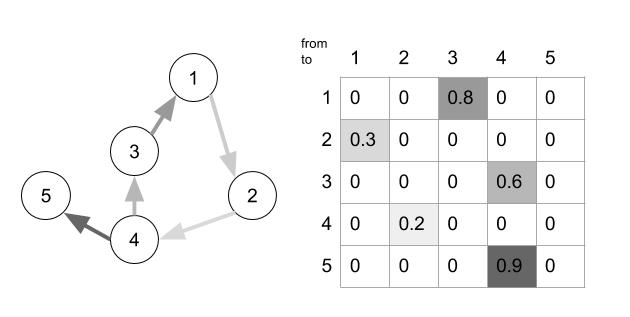
\includegraphics[width=0.49\textwidth]{images/directed_weighted_graph}
	 &
	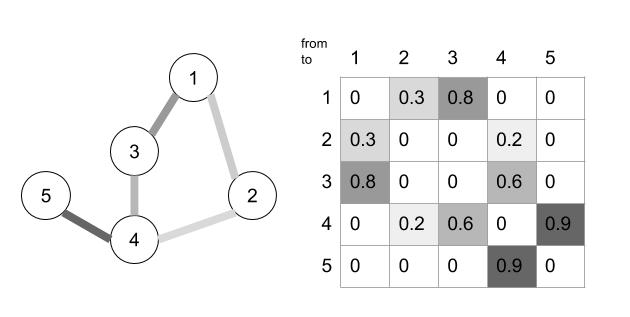
\includegraphics[width=0.49\textwidth]{images/undirected_weighted_graph} \\
	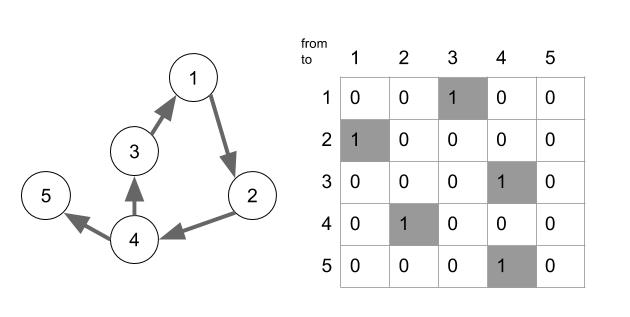
\includegraphics[width=0.49\textwidth]{images/directed_graph}  &
	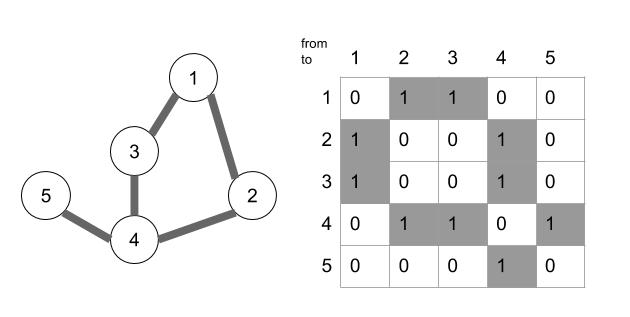
\includegraphics[width=0.49\textwidth]{images/undirected_graph} 
\end{tabu}
\captionof{figure}{4 different types of graphs (top: weighted directed and undirected, bottom: unweighted directed and undirected)\label{fig:graph_types}}
\end{table}


\subsection{directed/undirected}

Undirected edges may be traversed in any direction, whereas directed edges may just be traversed in one direction. For matrix representation of graphs, neither the mathematical \textbf{quiver}, a directed graph which has multiple arrows pointing from node $x$ to $y$, nor the \textbf{multigraph}, which is a graph which contains multiple undirected edges connecting just two nodes, is used.


\subsection{weighted/unweighted}

For graphs without costs defined for their edges, so called \textbf{unweighted graphs}, may be processed differently: 
\begin{itemize}
\item Either the algorithm searches for the shortest path, thus defining a uniform cost on all edges
\item Or there is no cost calculation at all, even the amount of edges is ignored
\end{itemize}

When adding weights to the edges, the graph is called a \textbf{weighted graph}. These weights typically represent different things, for example:
\begin{itemize}
\item time
\item length
\item energy consumption
\item elevations
\end{itemize}
to name just a few.

With weights defined on the edges, the approaches of algorithms are different, as the shortest path, in despite of number of traversed edges, is not necessarily the cheapest one. 



\section{Use cases}
Some use cases of the different graph types are (to name just a few examples):
\begin{itemize}
\item Navigation system (weighted directed)
	\begin{itemize}
		\item Nodes: Cities/POIs
		\item Edges: Routes directed (one way streets)
		\begin{itemize}
			\item weights
			\begin{itemize}
				\item length of street (find shortest way)
				\item time to traverse the street (find fastest way)
			\end{itemize}		
		\end{itemize}
	\end{itemize}		
\item Subway map (undirected unweighted)
\begin{itemize}
	\item Nodes: stations
	\item edges: connection between stations
\end{itemize}
\item Relations of tweets (directed unweighted)
\begin{itemize}
	\item nodes: single tweet entry
	\item edges: references to other tweets
\end{itemize}
\end{itemize}


\section{Matrix representation of graphs}

When representing graphs in a matrix, an adjacency matrix is used. Adjacency matrices are structured with every row and every column represents one node. This leads to a N x N square matrix, where N is the number of nodes. 

These matrices show some patterns according to their corresponding graph but most times these patterns are not immediately visible. There are some techniques to reveal these patterns, all of them involving the reordering of the matrix.


\subsection{Reordering}

The main goal of reordering the matrix is to cluster the edges and thus reveal certain patterns. An example of this behaviour can be seen in figure~\ref{fig:reorder}. 

\begin{figure}[h]
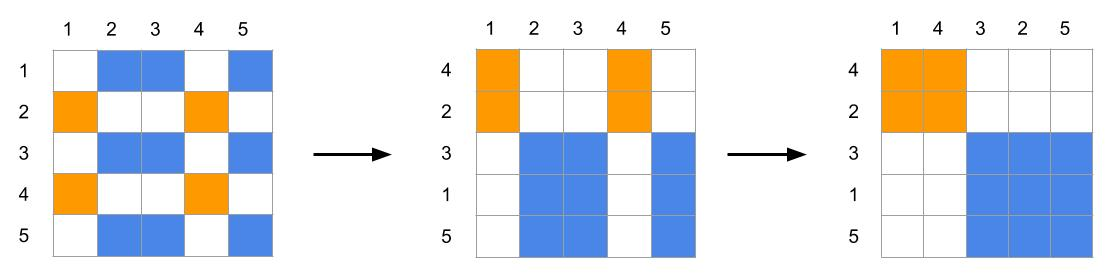
\includegraphics[width=\textwidth]{images/reorder}
\caption{Reordering a matrix\label{fig:reorder}}
\end{figure}


When reordering the matrix, the indices of the single rows and columns stay with the rows, otherwise the graph would change by this workstep. In this example, at first the rows 1 and 4 get swapped and as a second step columns 2 and 4. In this way the full connection pattern of the two subgraphs may be observed. 

\subsection{Patterns}
There are 4 main patterns which may be revealed by reordering the matrix. These patterns may be combined in such a way, that for example a subgraph creates a circle, but one node if it is connected to every other node. This results in a combination of the star and the circle pattern. 
The four different patterns can be seen in the corresponding figures~\ref{fig:patterns}.

\begin{table}[H]
  \centering
\begin{tabu}{cc}
	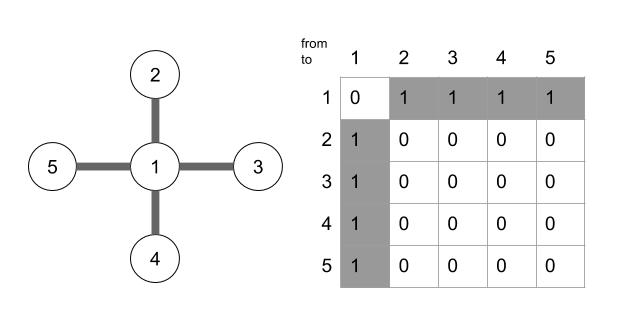
\includegraphics[width=0.49\textwidth]{images/pattern_star}  &
	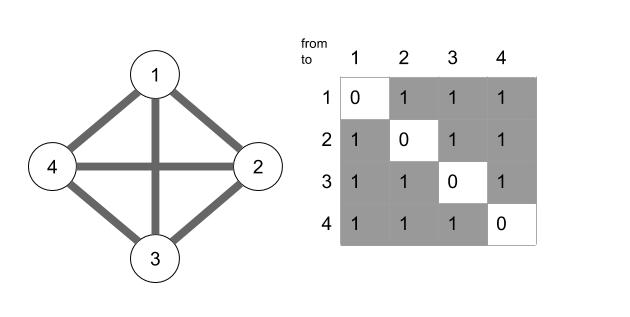
\includegraphics[width=0.49\textwidth]{images/pattern_full} \\
	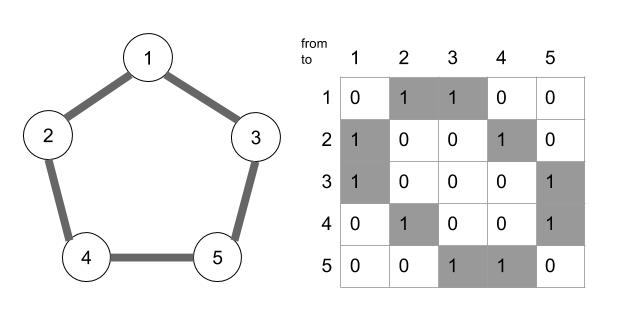
\includegraphics[width=0.49\textwidth]{images/pattern_circle} &
	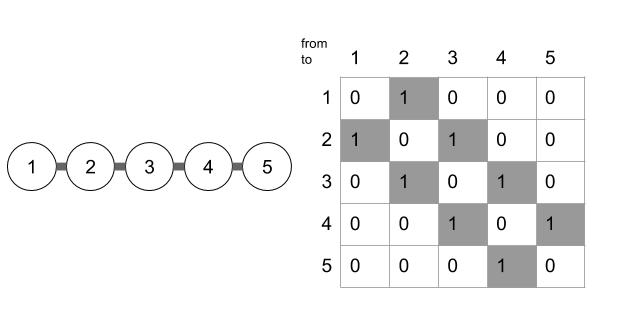
\includegraphics[width=0.49\textwidth]{images/pattern_line} 
\end{tabu}
\captionof{figure}{4 differnet patterns: star, full, circle and line\label{fig:patterns}}
\end{table}



\cleardoublepage
\chapter{Scalability}
\label{chap:Scalability}

Graph visualizations are always limited by the number of nodes, as well as the number of edges. The patterns in \ref{fig:patterns} can only be recognised if completely visible, therefore the hole adjacency matrix must be visible to find all of them. Otherwise patterns may not be entirely visible. This chapter gives an overview of the scalability of adjacency matrices, by estimating the upper limit of nodes in full visible adjacency matrix visualisations, explaining the problems of non full visible matrix visualisations, and reviewing the implementations Matrix zoom \cite{ham} and Nodetrix \cite{henry}.


\section{Maximum number of nodes in full visible adjacency matrices}
A short best case estimation will show the scalability limits of full visible adjacency matrix visualisations. Assuming all patterns should be recognisable, the hole matrix must be visible at once. Given a screen size of 25”, the number of nodes depends on the size of column, row and cell size. The number of displayable edges is in adjacency matrixes is always $|nodes|^2$.

Size of cells, rows and columns is determined by the their requirements. Pure visibility, intractability, or permanent visible node labels, or edge weights (cell labels) require increasingly more space.
If only a visible mark is required for an edge, a pixel is the lower limit for the marks size, otherwise marks can not be associated to the source or destination edge. Hi resolution screens do not increase the maximum number of nodes, since it is getting very hard to follow the grid lines to other nodes. By the way: my dsit trauma wants me to calculate the entropy of such matrix instance. Anyway, more than ~3000 nodes on a screen will cause a unreadable visualisation.
Mouse interactions like ‘on hover tooltips’ will add the option to identify source and destination nodes of an edge, but will also use more space and restrict the max nr of nodes. This will shrink the maximum number of nodes to ~300.
If edge node assoziation is an important task, permanent visible node labels in header will allow a interaction less visualisation of the graph. Additional space for labels reduces the maximum node code to 30.
 
 
\begin{table}[]
\centering
\begin{tabular}{|l|l|l|}
\hline
25" screen                 & max nodes & max edges                \\ \hline
Pixel grid                 & 3000      & $10^7$                     \\ \hline
Interactive cell or header & 300       & $10^5$                     \\ \hline
Labeled cell or header     & 30        & $10^3$                     \\ \hline
\end{tabular}
\caption{My caption}
\label{my-label}
\end{table}



\section{Non full visible adjacency matrices - zooming}
Putting a adjacency matrix in a zoom box obviously increases the maximum number nodes. 
When zoomed in, the readability of node and cell labels increases, but patterns may not be completely visible anymore. This requires the user to search the matrix by panning, a lot of panning. When zoomed out, labels are not readable anymore, and interactions with cells are impossible due to their small size. 

The following two section reviews Matrix zoom, a zoomable matrix visualisation which is avoiding these problems for clustered graphs. A general solution, without using known additional properties of the graph like the its clusters, was not found in the survey.

\section{Matrix subdivision}

Matrix zoom is a zoomable matrix visualisation \cite{ham}. It solves the label readability problem by finding new labels for groups of nodes or edges when zoomed out. It comes with a default dataset, describing a software repository. The nodes of the actual graph are function declarations and function calls of the source code, so it is the complete call graph of a software project. Classes, packages and layers are considered as clusters of the graph. 

When node labels get too small to read, they form groups by their containing classes, these groups are labeled with the class name. Multiple classes are represented by packages and so on. When edge marks get too small, a $n \times m$ block of edge marks is transformed to one cell, by calculating the density of the block and associating the cell color to to it.

\begin{figure}[h]
\centering
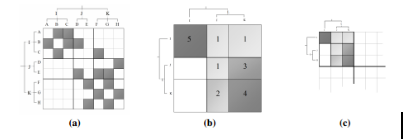
\includegraphics{images/matrixzoom_transform}
\caption{Reordering a matrix\label{fig:reorder}}
\end{figure}




\subsection{Cell and header transformations}   
This concept needs in general a way to transform blocks of labels to one label. The given example fits well to this requirement, since classes, packages are clusters and have human readable names. If the graph is clustered by algorithms, meaningful names of clusters must be found.

If other header visualisation techniques are used, the transformation must be adopted \ref{chap:headers}. For example if in or out degrees are visualized in the header, the average degree might be visualized by the group.

Transforming cell blocks to a cell can be done in various ways. If just the existence of an edge is relevant, the group cell may be rendered like a edge if at least one edge is in the cluster. Average weight, density or degree may also be relevant. Which of this transformations should be used is dependent on the requirements of the application, however, only one can be chosen.










\subsection{Recursive Matrix subdivision}   
\subsection{Sorting and clustering}   

Improvments in a spezific kontext, 
Clustering, recursive clustering: relations beteen nodes, clusters (ham). depends on clustering, this is dataproprocessing from my point of view.

Minimizing edgemarks not fitting in on screen, rduces the problem, but 
Arch graph


Hybrid: dens clusters (nodetrix) is usefull if dense subclusters a present. Shows them as adjm in traditional graph


\section{Hybrid Representation}
shows adjm in tratitionsl graph
best for dense clustes in graph


\cleardoublepage
%----------------------------------------------------------------
%
%  File    :  survey-style.tex
%
%  Author  :  Keith Andrews, IICM, TU Graz, Austria
% 
%  Created :  27 May 93
% 
%  Changed :  19 Feb 2004
% 
%----------------------------------------------------------------


\chapter{Cell Visualization Techniques}\label{chap:celltypes}


\section{What to visualize in cells?}
Often graph node links contain additional data, besides their connected nodes and weight, for example the textual description.

Most of the time, the cell simply represents the connection between two nodes by filling the cell. If the input is a weighted graph, this information is often extended by the edge weights. Given the case that the input graph is undirected, the cells form a symmetric pattern along the diagonal. 

On the other hand, the cell can also represent data of a node, for example the affiliation to a specific cluster or the similarity to nodes from other clusters or the local neighbourhood. 
Most tools provide the possibility to highlight the current selection in the matrix.

\section{How to visualize it in cells?}

Connections are most of the time shown in a black-white scheme, where black means that there is a connection, and accordingly white shows, that there is none. The current selection is then highlighted by increasing the transparency of the not-selected cells or simply setting them to grey. The logical next step from this is the extension to a wider color scheme, so that for example weights can be represented by different color grades, additionally with text as a fallback. If this scale is discrete, there is also the possibility to display icons or textures instead of color grades.
If the data which should be visualized is more exotic, like the similarity of nodes in the local neighbourhood, this could be displayed as bar charts or histograms inside the cells. A matrix cell can even include another matrix and represent the according sub-cells. This technique is mainly used to simplify complex and large matrices.


\section{Example: Nodetrix}


\begin{figure}[H]
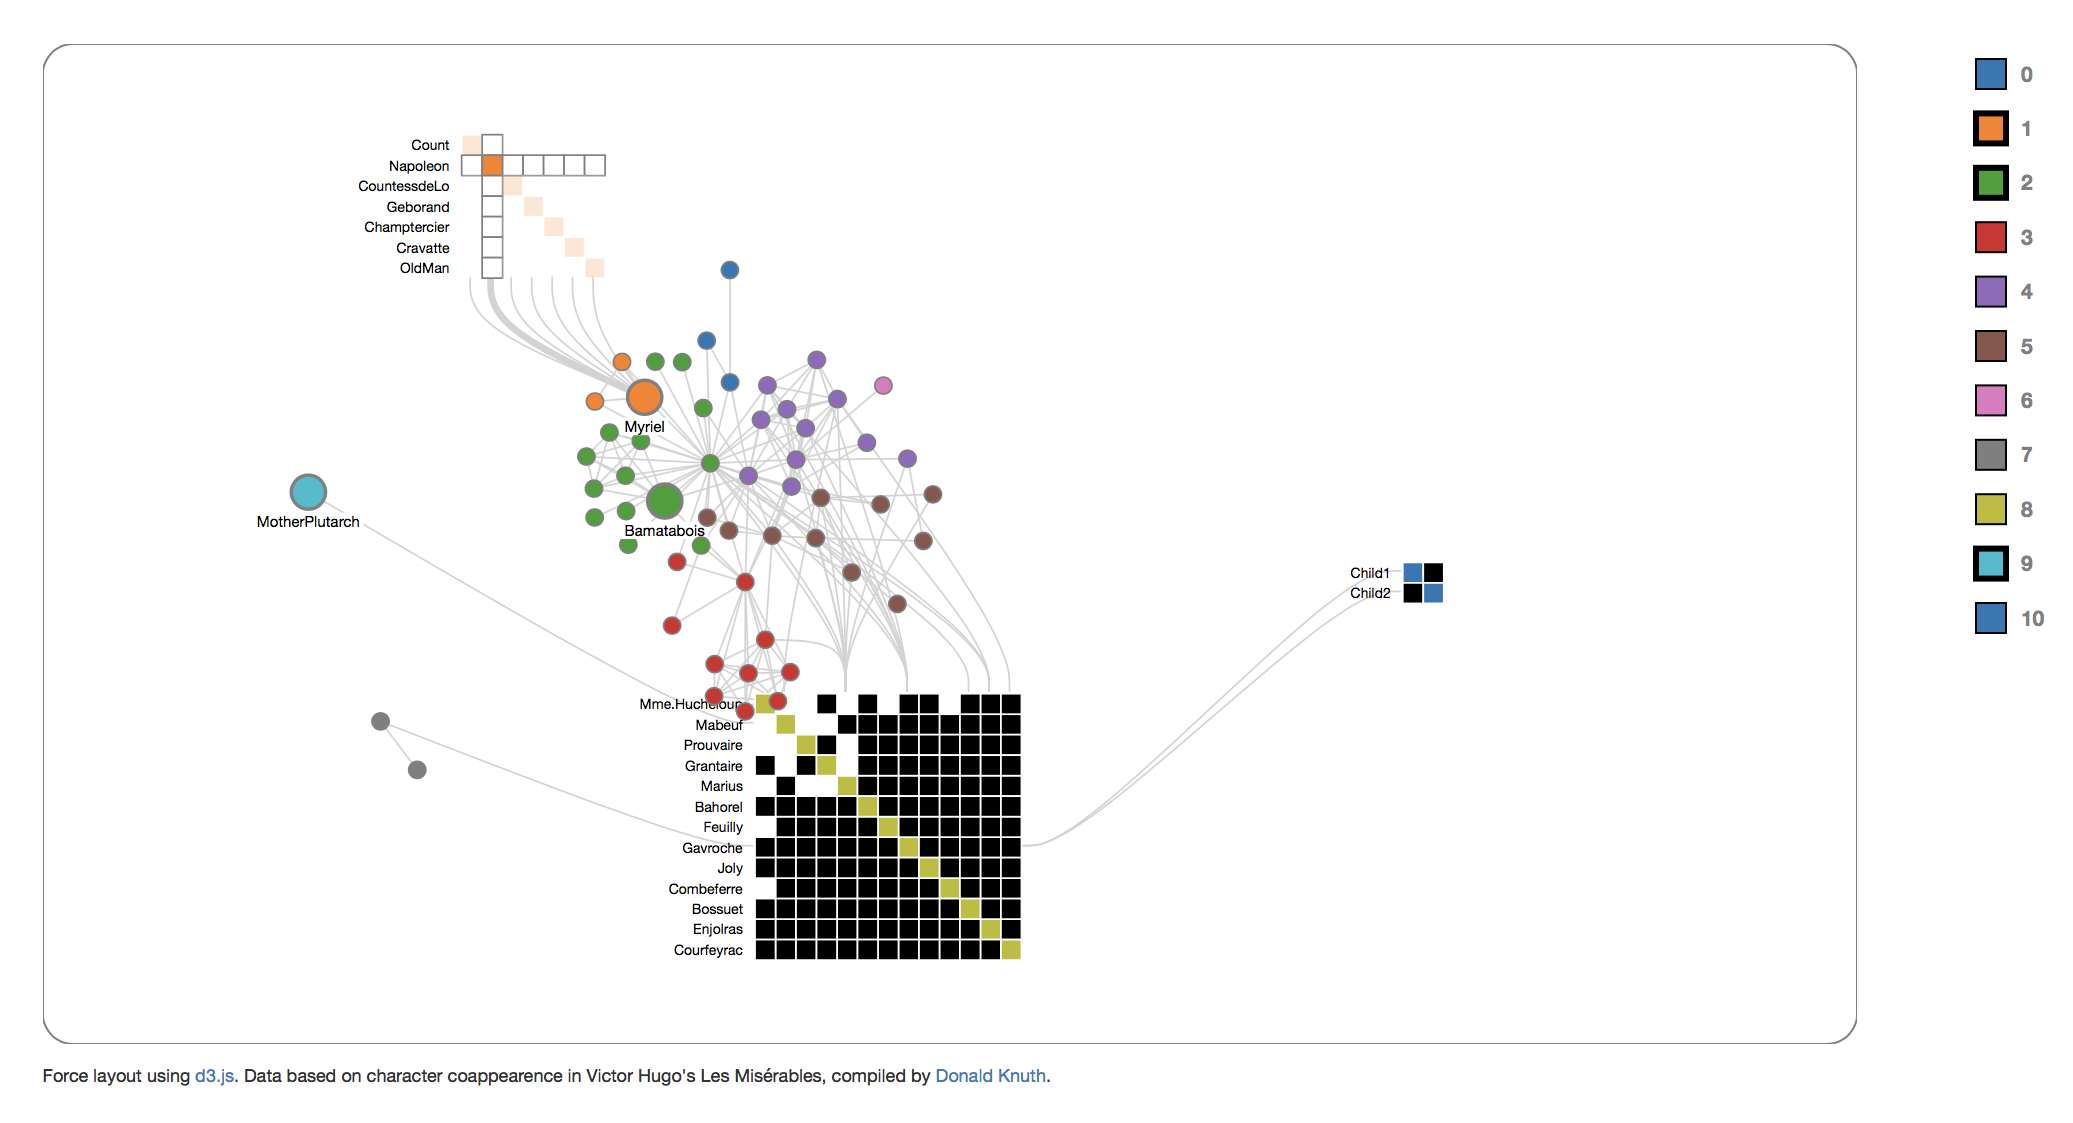
\includegraphics[width=\textwidth]{images/nodetrix_cell}
\caption{TODO: Screenshot created using Nodetrix...\label{fig:cell_nodetrix}}
\end{figure}



In the matrix representation of Nodetrix, connections are shown as black cells, the color in the matrix diagonal visualizes the affiliation to a specific cluster in the graph. The matrices in Nodetrix have a hover effect, which highlights the row and column of the currently selected cell. Every other cell in the matrix becomes light gray to help the user focus on connections. Additionally, the connections to graph nodes from the selected cell are emphasized too, as they are drawn boldly. 

\section{Example: Matrix Zoom}


Matrix zoom uses colors to visualize edge attributes. In the example set, edge attributes are an indication if a call is allowed or not or the local neighbourhood of a call, visualized in a color scale. Therefore, calls, which have a shorter path-distance to the considered call are indicated in red. Transparency is used to indicate the call density of this matrix cell, higher cell density meaning a larger percentage of subcells containing calls. TODO: citation ham-ivis2003.pdf


\begin{figure}[H]
\centering
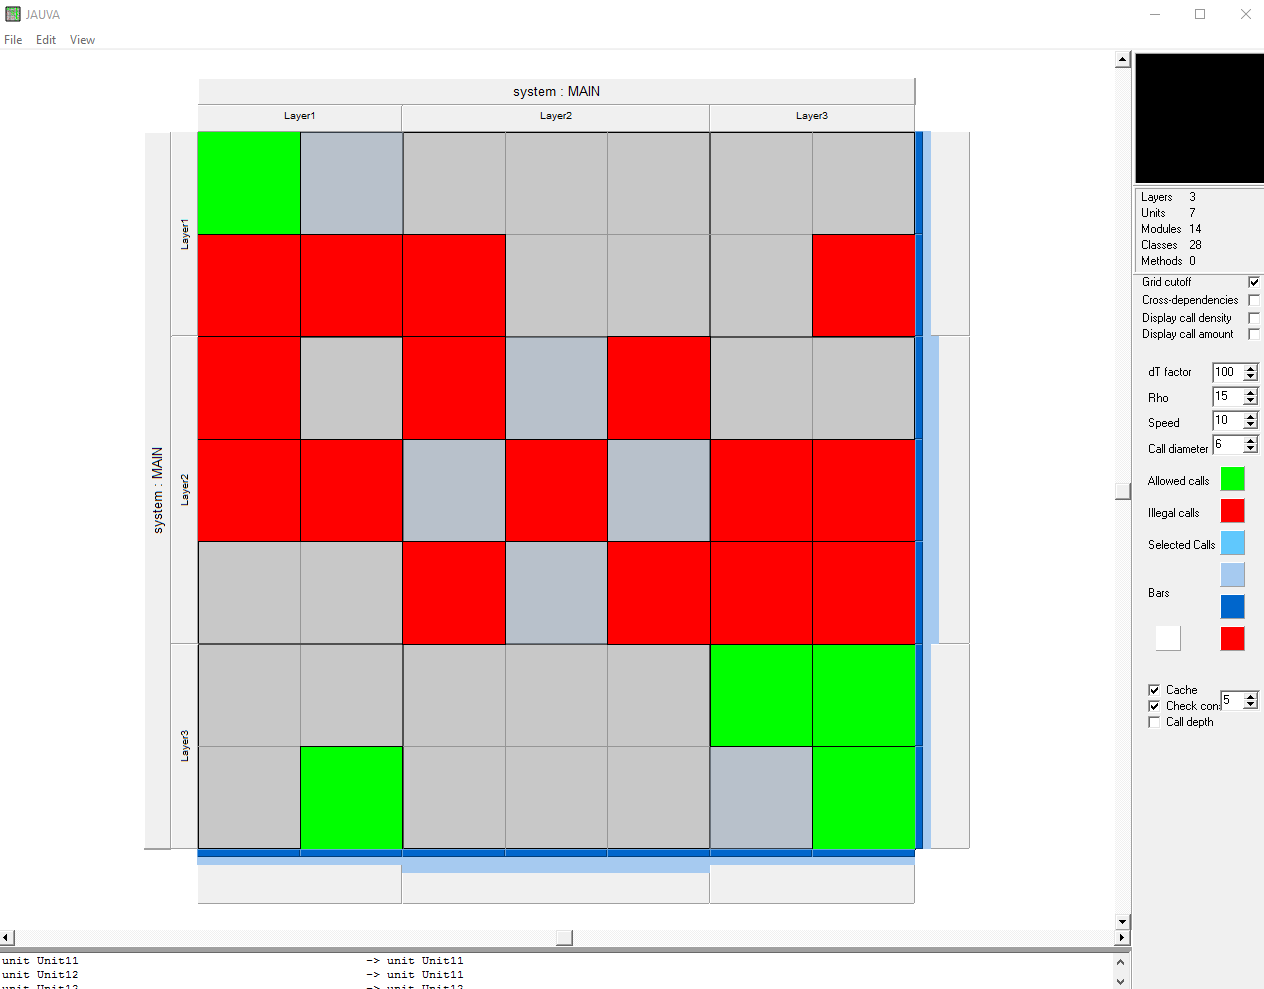
\includegraphics[width=0.8\textwidth]{images/matrixzoom_cell}
\caption{Screenshot created using Matrix zoom...\label{fig:zell_matrixzoom}}
\end{figure}


\section{Example: Cubix}

\begin{figure}[H]
\centering
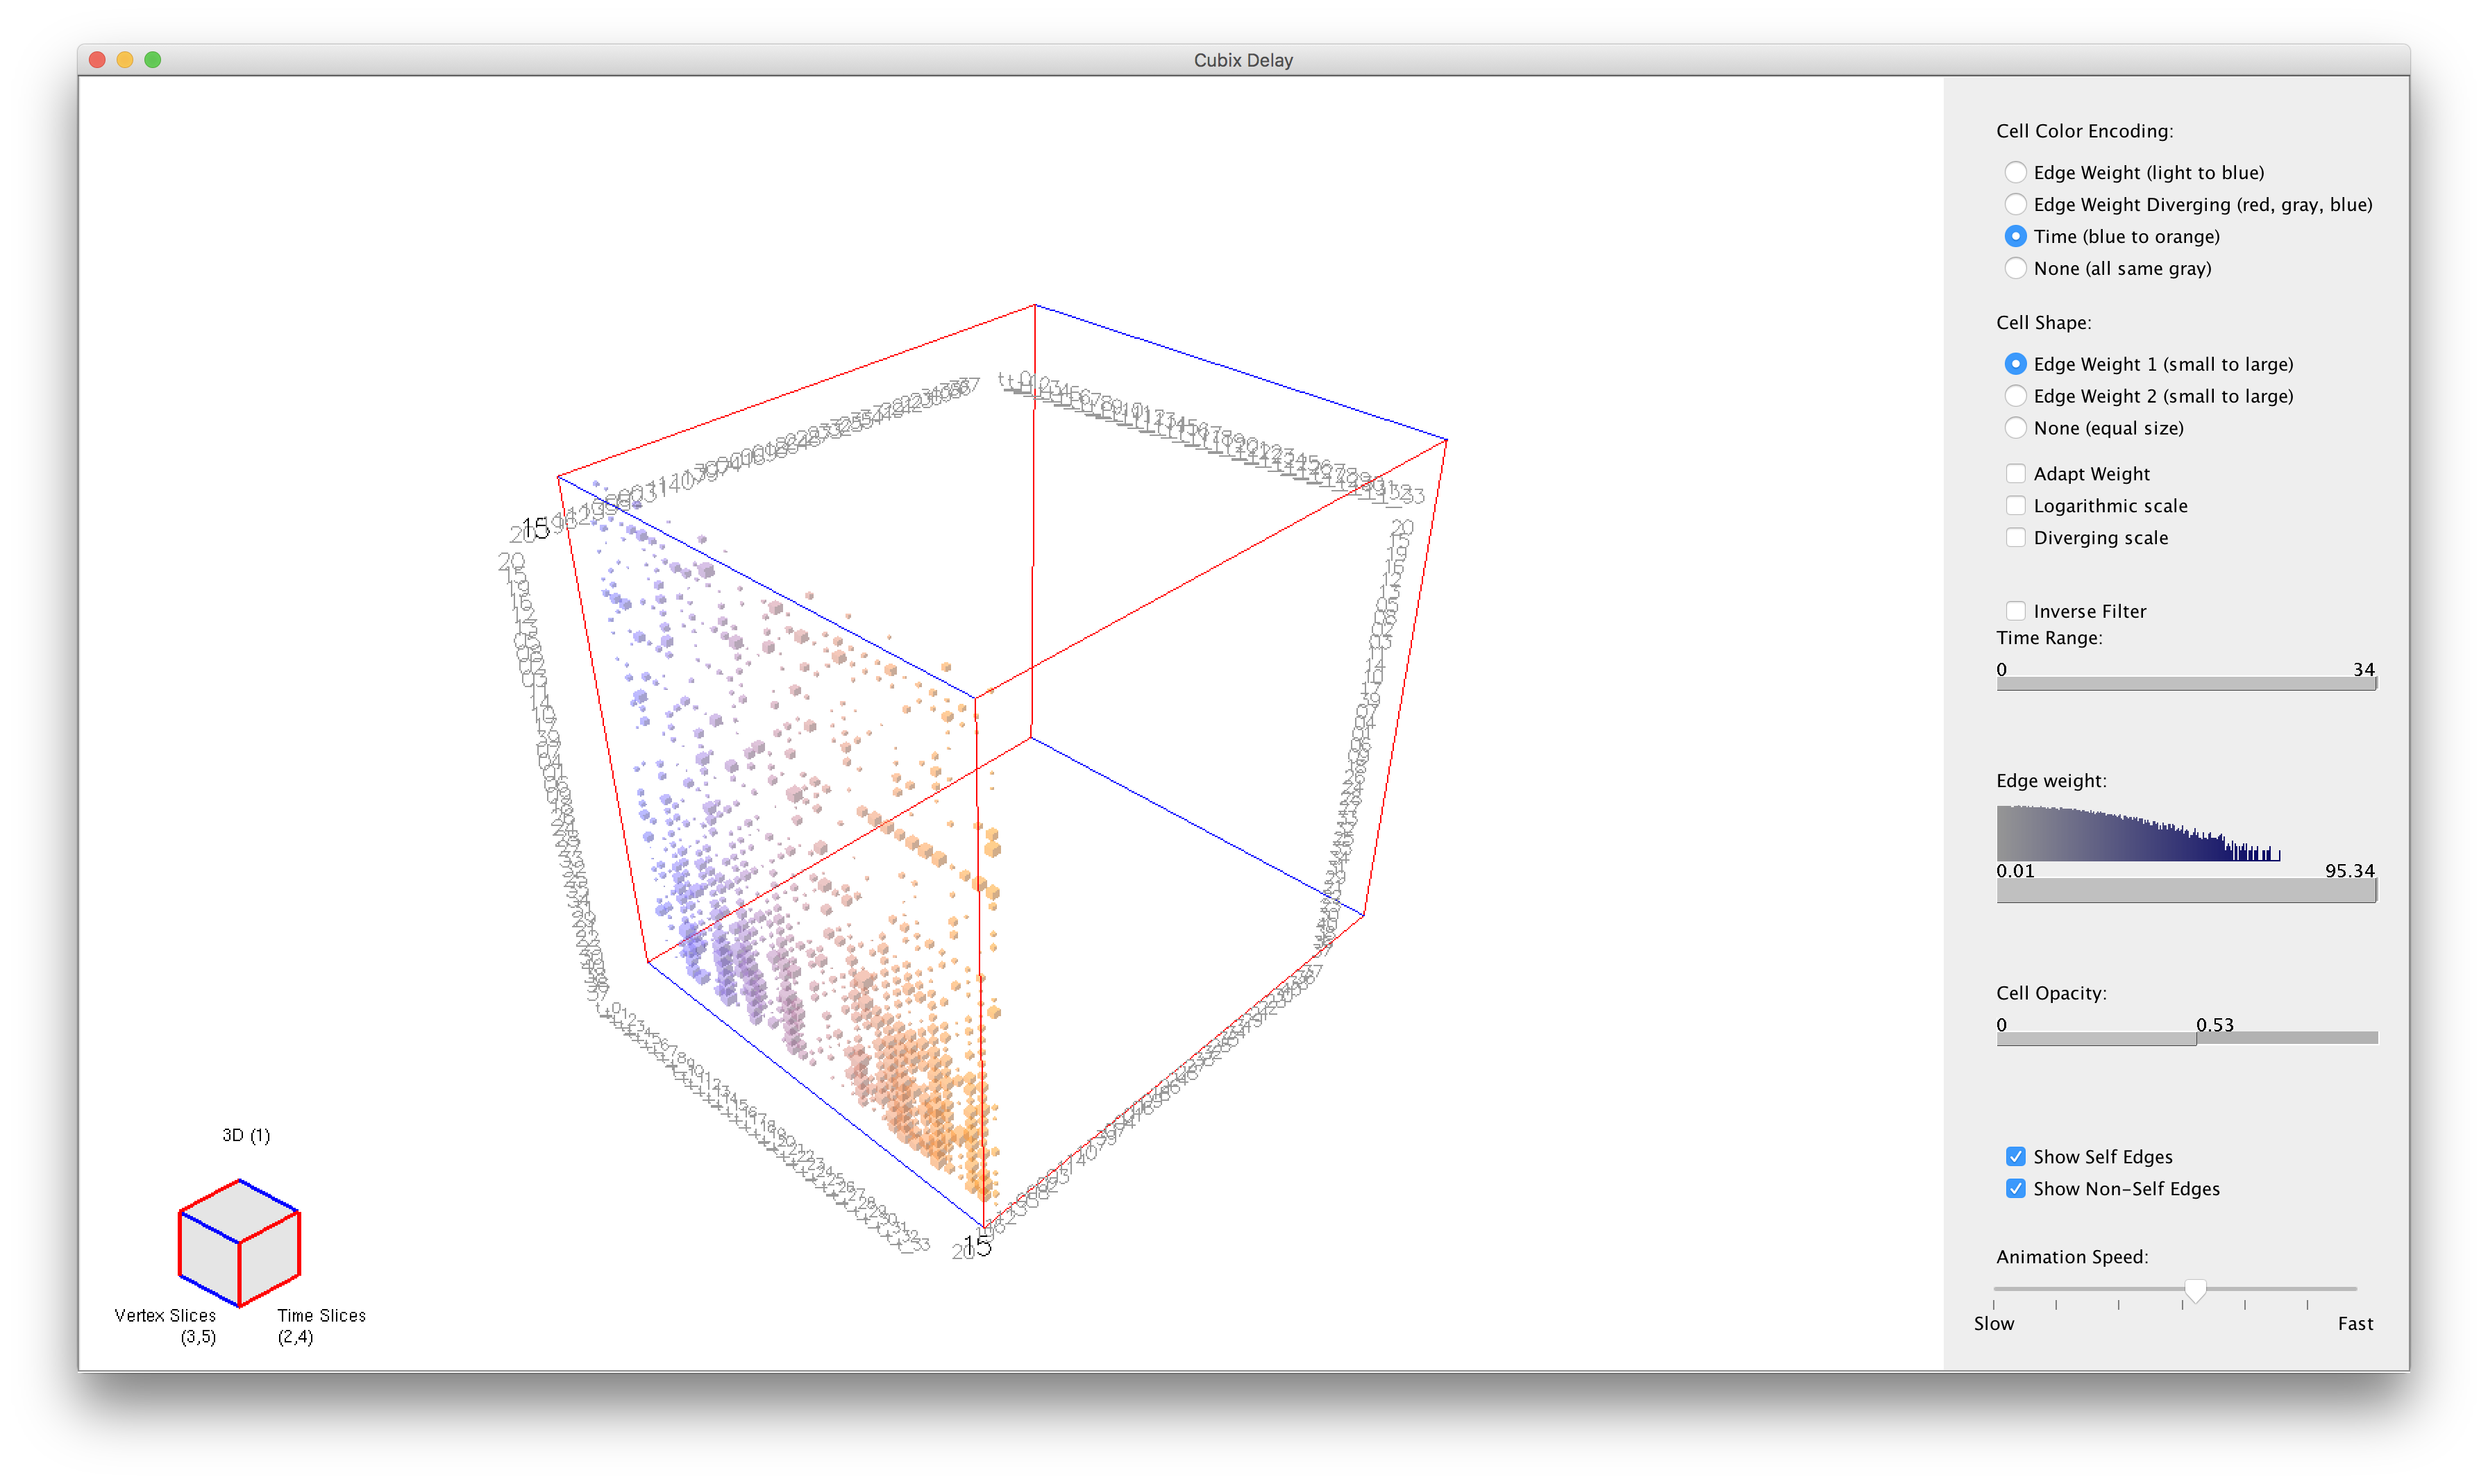
\includegraphics[width=0.8\textwidth]{images/cubix3d_cell}
\caption{The 3D representation of Data in Cubix, screenshot created using Cubix\label{fig:cell_cubix3d}}
\end{figure}

\begin{figure}[H]
\centering
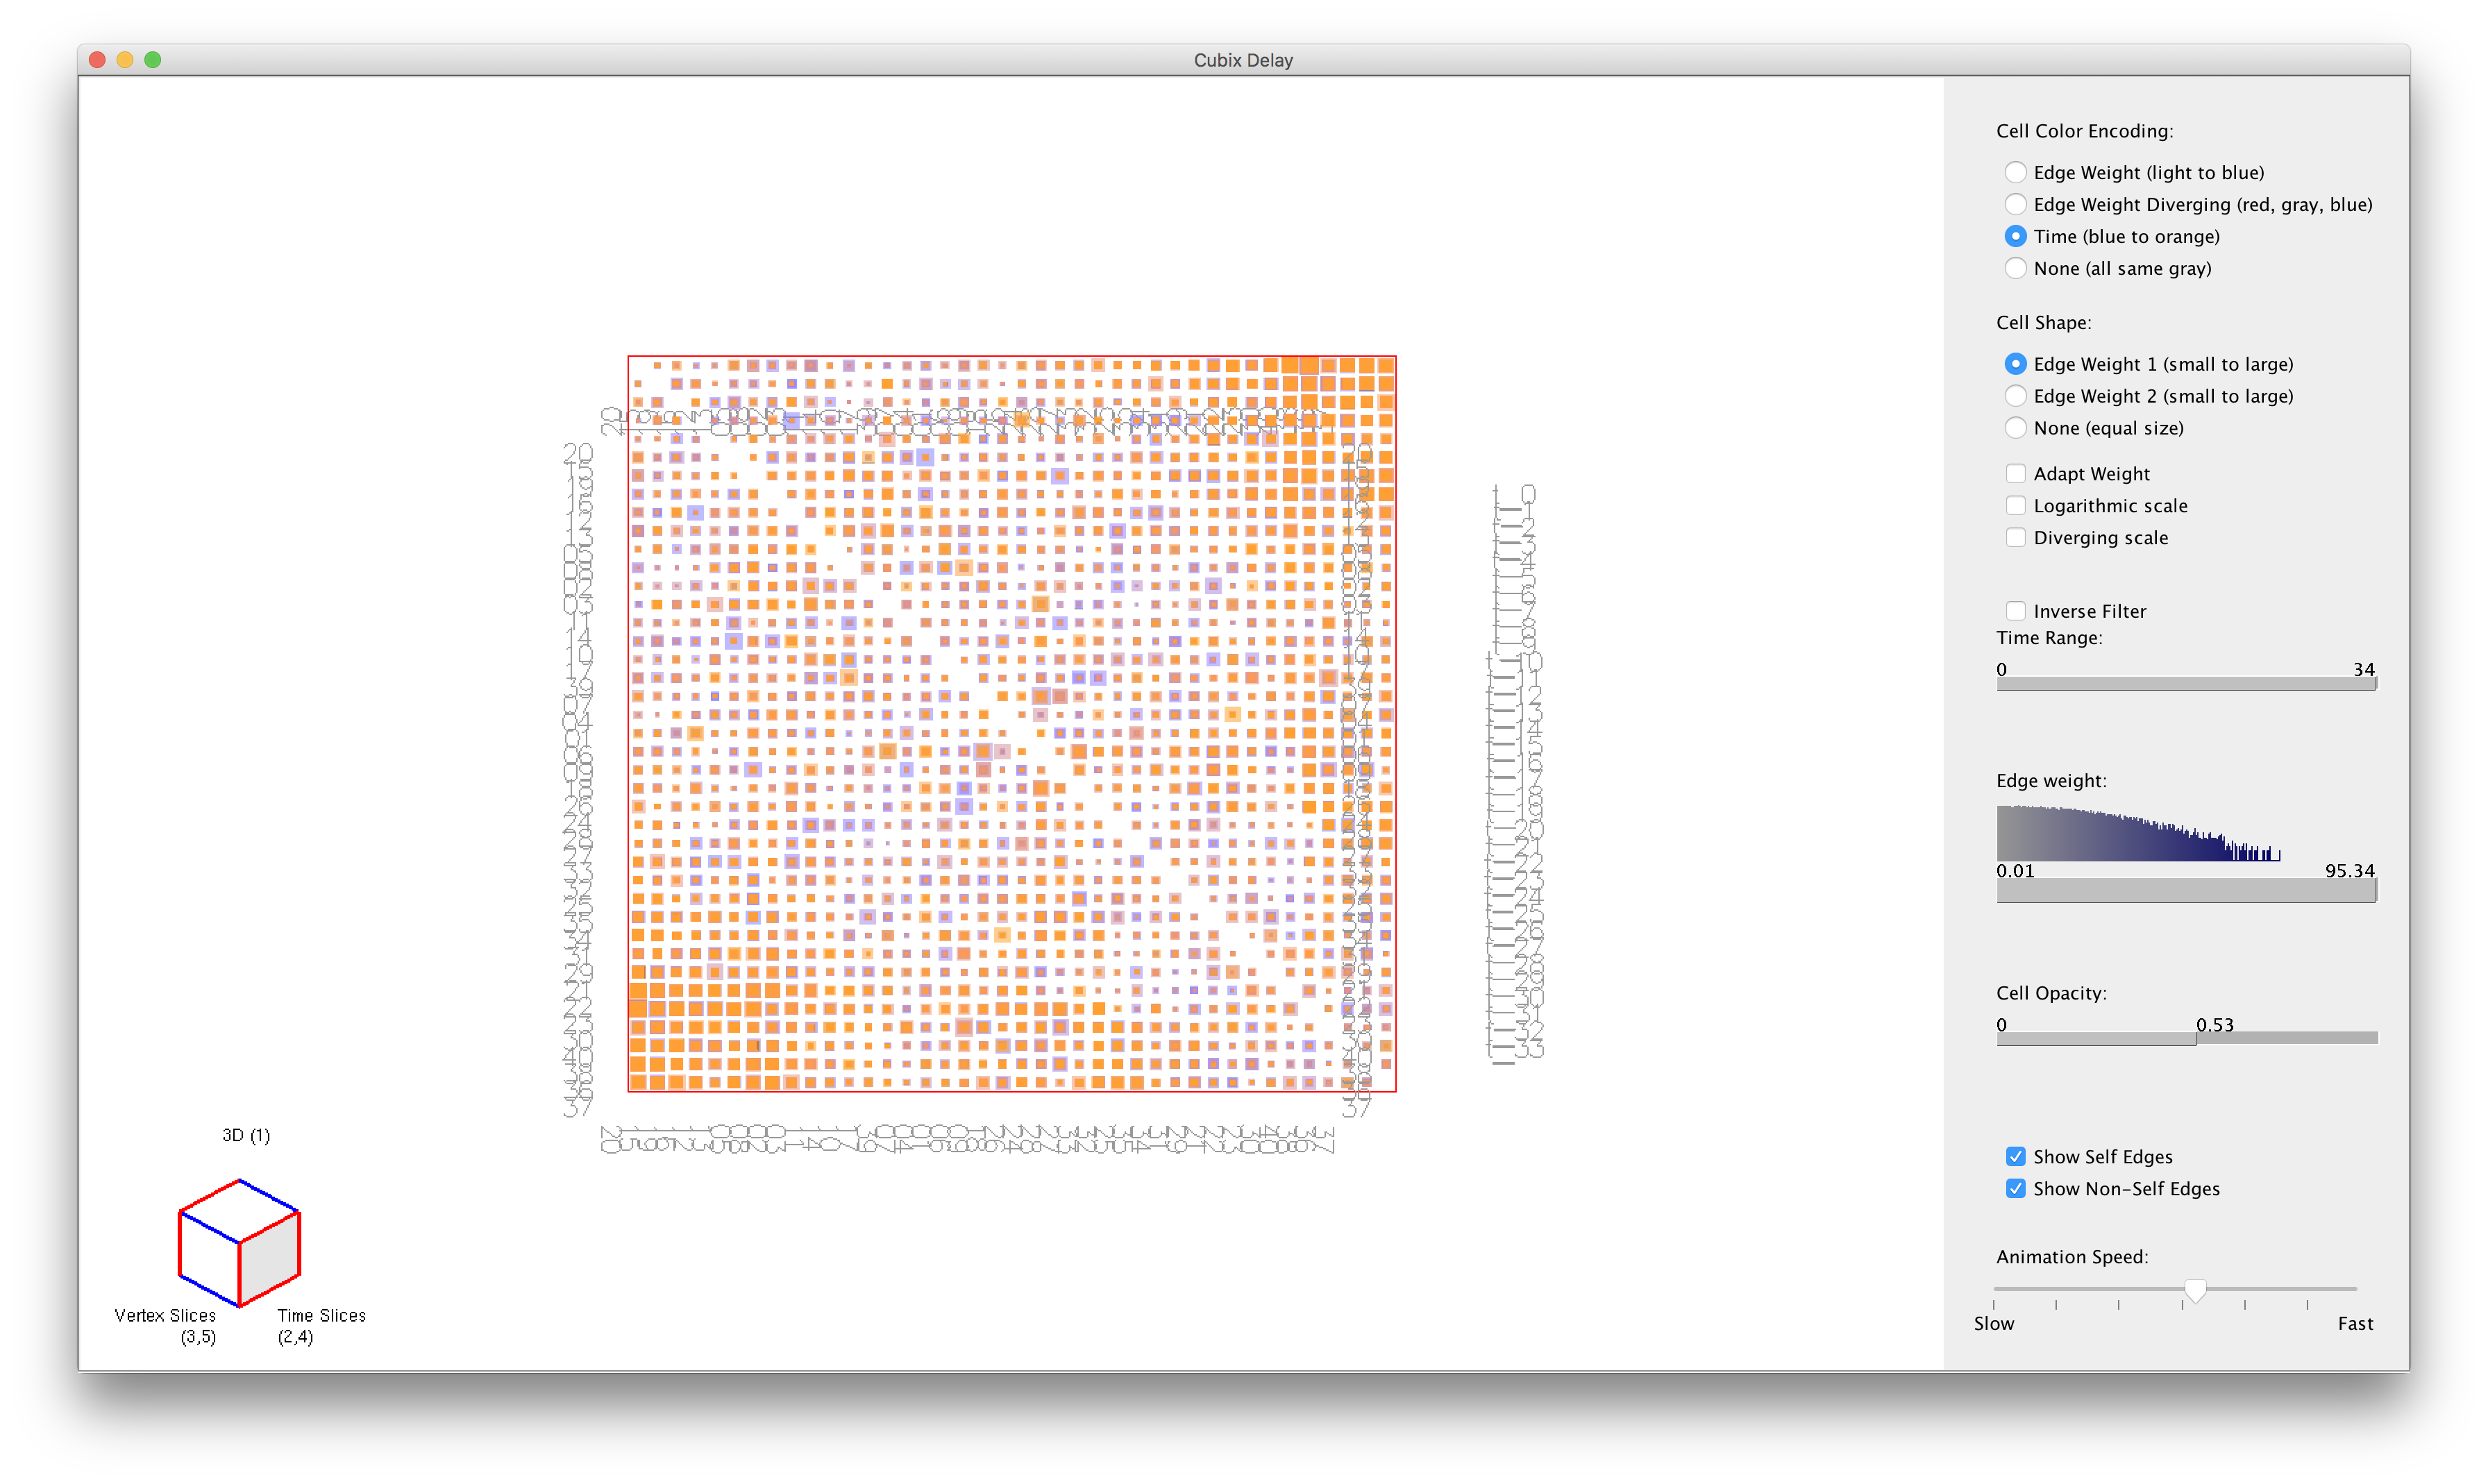
\includegraphics[width=0.8\textwidth]{images/cubix2d_cell}
\caption{The same data in 2D shown as time slices, screenshot created using Cubix\label{fig:cell_cubix2d}}
\end{figure}


Cubix is a tool to visualize and analyze graphs, which changes over time using the space-time-metaphor. Adjacency matrices are stacked onto each other in chronological order to create a cube with two vertex and one time dimension.

The cell colors represent by default the edge weight, this can also be changed to the edge weight diverging or the affiliation to a specific time slice. The user can switch off the color encoding too, for easier recognizing patterns of the cells. Since this is a three-dimensional visualization, cell opacity is an important method for identifying patterns or cells behind another one. 

Additionally, the size of the cell is another tool to visualize the weight of the edges and their change over time. For pattern finding, this feature can also be turned off. TODO: citation Bach2014cubix.pdf (http://www.aviz.fr/~bbach/cubix/Bach2014cubix.pdf)



\cleardoublepage
%----------------------------------------------------------------
%
%  File    :  thesis-tech.tex
%
%  Author  :  Eva Rott, TU Graz, Austria
% 
%  Created :  14 May 2017
% 
%  Changed :  16 May 2017
% 
%----------------------------------------------------------------


\chapter{Reordering}\label{chap:reordering}

Reordering describes the process of either moving nodes in a graph or moving rows or columns in a matrix. There are two types of reordering: manual and automatic. Manual reordering is done by the user of a software. This survey focuses on automatic reordering, which is done by a software tool based on its implemented algorithms. The information used as input for the algorithms can be the node label, node in / out degree or clustering data. The mentioned information sources are not a complete list of available reordering input data. However, they were found in the tested programs and they are described in more detail in the following enumeration.

\begin{enumerate}
	\item Reordering using node label. The data used for this example describes a number of functions of a program connected corresponding to the its control flow. Figure $[function_calls_graph.png]$ TODO shows the directed graph with the functions as nodes; Figure $[sample_matrix.png]$ TODO the unsorted matrix representation of the graph. The result of reordering the matrix based on alphabetic label name order can be seen in figure $[reordered_by_label.png]$ TODO.
	
	\item Reordering using node out degree. The data used for this example is the same as in TODO. Figure TODO shows a reordered matrix based on ascending order of node in and out degree. The function with the largest number of incoming links is the rightmost column and the node function with the largest number of outgoing links the lowermost row of the matrix.

	\item Reordering using node clustering. As node clustering needs to be computed first, this type of reordering is explained in an example taken from the program Nodetrix. Displayed in figure TODO $[nodetrix_reordering.png]$ is the graph with the clustered nodes, marked in different colors, and some sub-matrices for some of the ordered clusters.
\end{enumerate}


\cleardoublepage
%----------------------------------------------------------------
%
%  File    :  thesis-tech.tex
%
%  Author  :  Eva Rott, TU Graz, Austria
% 
%  Created :  14 May 2017
% 
%  Changed :  16 May 2017
% 
%----------------------------------------------------------------


\chapter{Matrix Headers}
\label{chap:headers}

A standard matrix visualization contains a symmetric grid representing the node connections and node labels on top and to the left side of the grid. In this survey this area and in general the area around the grid is referred to as matrix header. The matrix header can be used for visualizing additional information about the matrix data. An example for that is a group of node connections, the node density or the current level of zoom in a multi-layer matrix.
There are various techniques to achieve additional information visualization in a matrix header. Most of them can be found in the program Matrix Explorer.

The Matrix Explorer is another tool for matrix visualization of graphs. As seen in figure \ref{fig:header_matrixexplorer}, the program displays the matrix without a zoom functionality, while giving a small overview of the full matrix in the top left corner of the graphical user interface. Aside from the matrix visualization, the Matrix Explorer provides various options for filtering and sorting of nodes and executing operations on the matrix headers. The following section describes the most common operations and gives one example per listed header visualization technique for a better understanding. 

\begin{figure}[tp]
  \centering
  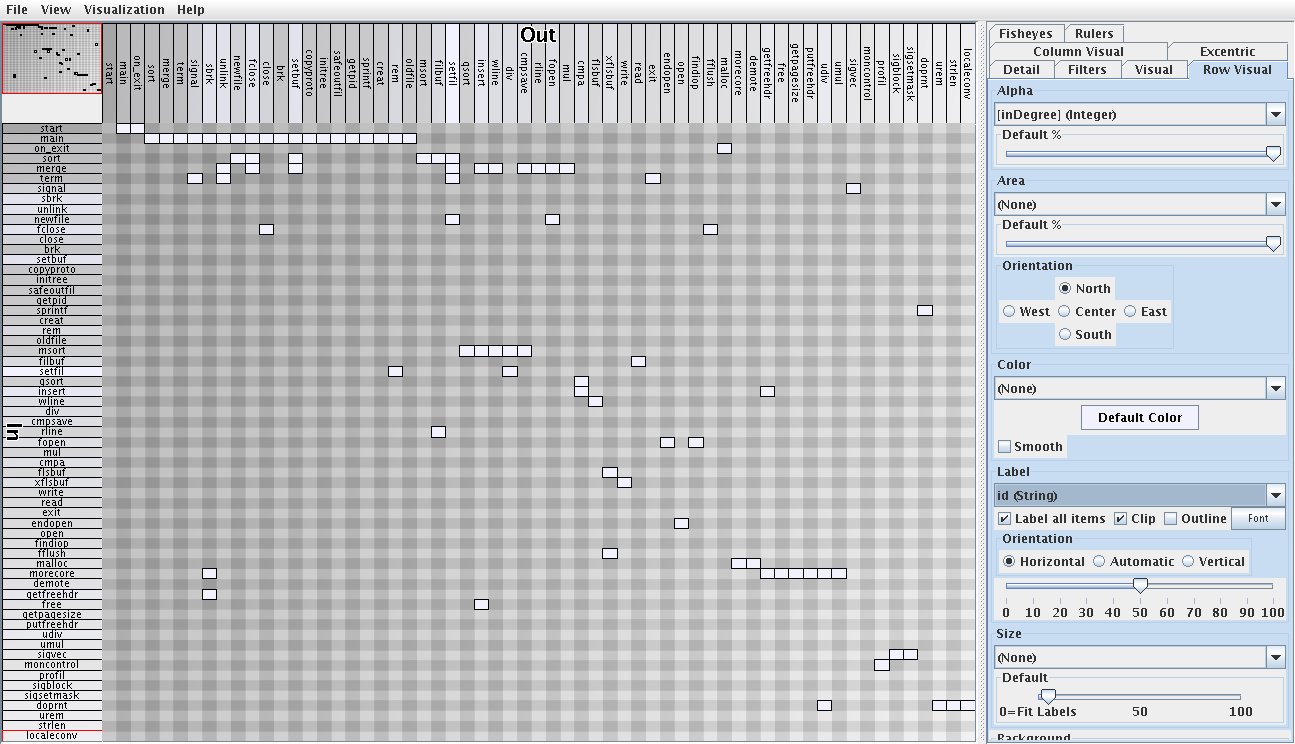
\includegraphics[keepaspectratio,width=\hsize,height=\halfh]
  {images/Header_MatrixExplorer.png}
  
  \caption[Matrix Visualization Tool Matrix Explorer]{
  The graphical user interface of the matrix visualization tool Matrix Explorer \citep{henry-phd-2008}.
  \imgcredit{Screenshot created by an author of this thesis using Matrix Explorer. \citep{henry-phd-2008}.}
  }
  \label{fig:header_matrixexplorer}
\end{figure}

\section{Node Connections}
As seen in figure \ref{fig:header_matlink} from the program MatLink, created by \citep[105-118]{henry-phd-2008} curved lines are used for highlighting node connections. The shortest path is highlighted in red. When one node is selected, the program draws the paths in the headers of the matrix. Using this visual information it can quickly be seen how many other nodes are connected directly to the selected node. In addition, the path from one node to another connected node can be traversed using these lines \citep[105-118]{henry-phd-2008}.

\begin{figure}[tp]
  \centering
  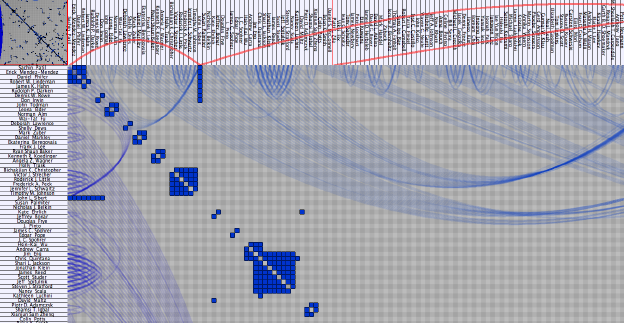
\includegraphics[keepaspectratio,width=\hsize,height=\halfh]
  {images/Header_MatLink_path.png}
  
  \caption[Highlighting Matrix Paths]{
  In the program MatLink \citep[105-118]{henry-phd-2008} the paths between selected nodes are highlighted using curved lines. The shortest path is drawn in red.
  \imgcredit{Image taken from the master thesis \citep[105-118]{henry-phd-2008}.}
  }
  \label{fig:header_matlink}
\end{figure}

\section{Histogram per Node}
\label{sec:histogram-per-node}
A histogram can be computed over various node properties. An example for such a property is the node degree. The Matrix Explorer offers this histogram functionality. Figure \ref{fig:header_matrixexplorer_histogram} shows a matrix visualization of data similar to that used for the first two examples in the previous chapter. Again, a set of functions from a program are represented as nodes and the programs control flow as links. Looking at the histogram which was computed over the outgoing links it becomes obvious that the main function has the largest light gray area. This means that it has the largest number of outgoing links of all nodes. In contrast to the node out degree distribution, the incoming links follow a more balanced distribution. Considering this example, a histogram in the header is well suited for showing the general distribution of the node degree. In case nodes containing extreme values should be highlighted, the header color visualization technique can be used.

\begin{figure}[tp]
  \centering
  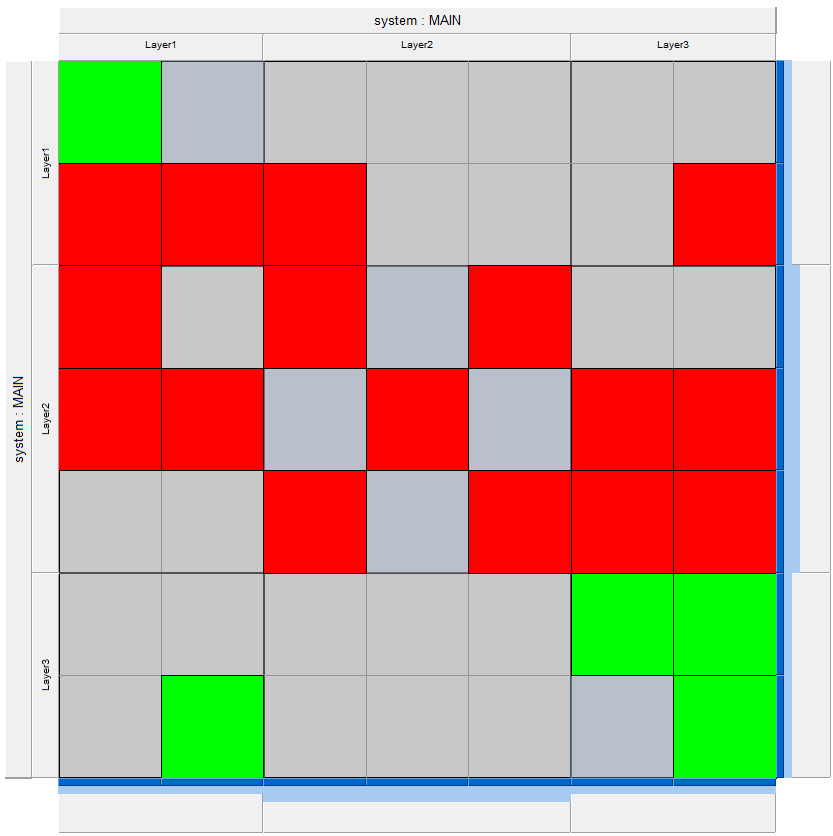
\includegraphics[keepaspectratio,width=\hsize,height=\halfh]
  {images/Header_MatrixExplorer_histogram.png}
  
  \caption[Matrix Header with Histogram of Node Degree]{
  The size of the white area in the node label represents the node degree.
  \imgcredit{Screenshot created by an author of this thesis using Matrix Explorer. \citep{henry-phd-2008}.}
  }
  \label{fig:header_matrixexplorer_histogram}
\end{figure}

\section{Color Highlighting}
Every node in a graph can be assigned a color in a certain range. This color distribution assigned to the nodes can be computed for the same properties as the histogram. The darker the color the higher the value of this node. Considering the same example and figure \ref{fig:header_matrixexplorer_color} as in the previous section, it becomes obvious that the start function has no incoming links as it is the root function of the program.

\begin{figure}[tp]
  \centering
  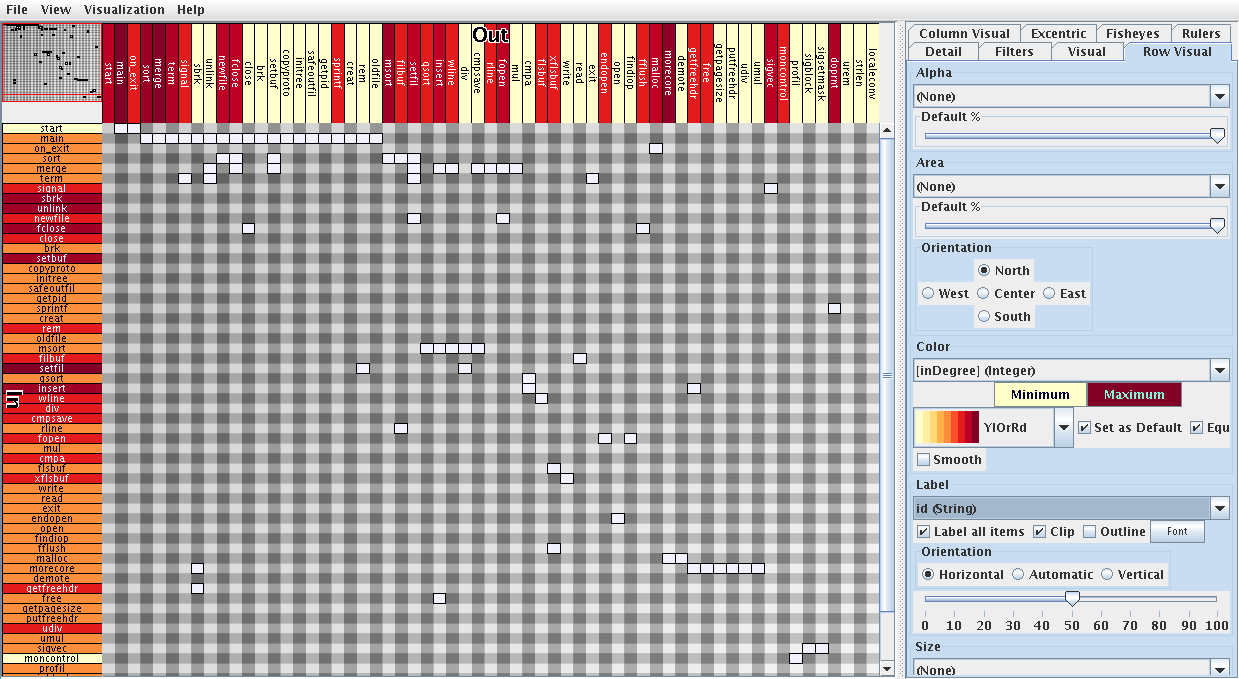
\includegraphics[keepaspectratio,width=\hsize,height=\halfh]
  {images/Header_MatrixExplorer_color.png}
  
  \caption[Matrix Header with Color Representation of Node Degree]{
  The intensity of the color in the node label represents the node degree.
  \imgcredit{Screenshot created by an author of this thesis using Matrix Explorer. \citep{henry-phd-2008}.}
  }
  \label{fig:header_matrixexplorer_color}
\end{figure}

\section{Histogram per Matrix Sub-Section}
In contrast to the histogram computed per node as explained in \ref{sec:histogram-per-node} , a histogram can also be computed over multiple columns or rows at the same time. Figure \ref{fig:header_matrixzoom_histogram} shows an example. The screenshot was taken from the matrix visualization program MatrixZoom. The displayed matrix is divided into three times three sub-sections. For every group of three vertically or horizontally aligned sections the amount of data contained in it is computed. Next, those values are transformed into a histogram representation, which is then drawn as light blue bars on the right and bottom matrix header. The result shows that the center section of the matrix has the largest density of data points of all sub-sections.

\begin{figure}[tp]
  \centering
  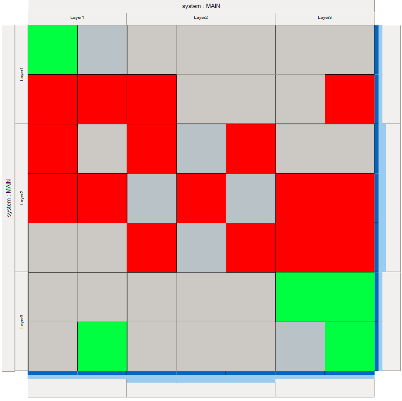
\includegraphics[keepaspectratio,width=\hsize,height=\halfh]
  {images/Header_MatrixZoom_histogram.png}
  \caption[Matrix Header with Histogram of Matrix Section Density]{
  The matrix is divided into nine different sub-sections. For each row and column of sub-sections the density of data points is computed. The result is drawn as light blue bars in the right and bottom matrix header.
  \imgcredit{Screenshot created by an author of this thesis using Matrix Zoom. \citep{ham2005phd}.}
  \label{fig:header_matrixzoom_histogram}}
\end{figure}


\cleardoublepage
\setcounter{secnumdepth}{-1}
\chapter{Conclusion}
Several tools for matrix visualization of graphs were discussed and evaluated with focus on the implementation of a zoom function, cell visualization techniques and matrix header visualizations. Evaluating all of these three points, it became clear that each of the presented tools implements a different key aspect. While MatrixZoom has the best zoom implementation, Nodetrix provides very good cell visualization techniques, Matrix Explorer offers the best support for additional information visualization. 

All in all, no program can be recommended in general for any application. Best approach is to consider the type and size of the data before choosing a matrix visualization tool.

\cleardoublepage
\printbibliography[heading=bibintoc]

\end{document}

